\chapter{The Molecular Chaos Transport Circle}\label{ch:kinetic}

\section{Chapter aim and attribution}
This chapter reconstructs a geometric consequence of the analytical transport coefficients derived by Allocca \etal\ for a chiral FHP cellular automaton \cite{Allocca2026}. The continuum coefficients and the underlying kinetic derivation are attributed to that work. The contribution here is the exact elimination, spectral rewriting, independent finite arithmetic verification, and the separation between that kinetic identity and the correlated problem studied later.

\section{Parameterization of the published coefficients}
Let $\rho$ be the mean occupancy density and let $p$ denote the probability that resolves the chiral collision choice in the published model. Introduce
\begin{equation}
 d=p-\frac12,
 \qquad
 D=\rho\left(1-\frac{\rho}{6}\right)^3.
 \label{eq:kin_D}
\end{equation}
Away from the singular endpoints $D=0$, define
\begin{equation}
 A=\frac{1}{2D},
 \qquad
 u=\frac{2\sqrt3}{3}d.
 \label{eq:kin_Au}
\end{equation}
The lattice contribution is most conveniently absorbed into the shifted shear coordinate
\begin{equation}
 \bar\eta=\eta+\frac18.
 \label{eq:eta_shift}
\end{equation}
The zero field transport formulas can then be written
\begin{equation}
 \bar\eta=\frac{A}{1+u^2},
 \qquad
 \eta_H=-\frac{Au}{1+u^2}.
 \label{eq:kin_coeffs}
\end{equation}
The parity symmetric point is $p=1/2$, where $u=0$ and $\eta_H=0$.

\section{Elimination of chirality}
Squaring the two expressions in \cref{eq:kin_coeffs} gives
\begin{align}
 \bar\eta^2+\eta_H^2
 &=\frac{A^2(1+u^2)}{(1+u^2)^2}\\
 &=\frac{A^2}{1+u^2}\\
 &=A\bar\eta.
 \label{eq:kin_circle_shifted}
\end{align}
Completing the square yields
\begin{equation}
 \left(\bar\eta-\frac{A}{2}\right)^2+\eta_H^2
 =\left(\frac{A}{2}\right)^2.
 \label{eq:kin_circle_centered}
\end{equation}
Returning to the unshifted coordinate,
\begin{equation}
 \left(\eta+\frac18-\frac{A}{2}\right)^2+\eta_H^2
 =\left(\frac{A}{2}\right)^2.
 \label{eq:kin_circle_eta}
\end{equation}
At each fixed density the kinetic response therefore lies on an arc of a circle in the $(\eta,\eta_H)$ plane. The radius and center depend on density through $A$. The curve traversed by $p\in[0,1]$ need not cover the whole circle.

\begin{figure}[htbp]
\centering
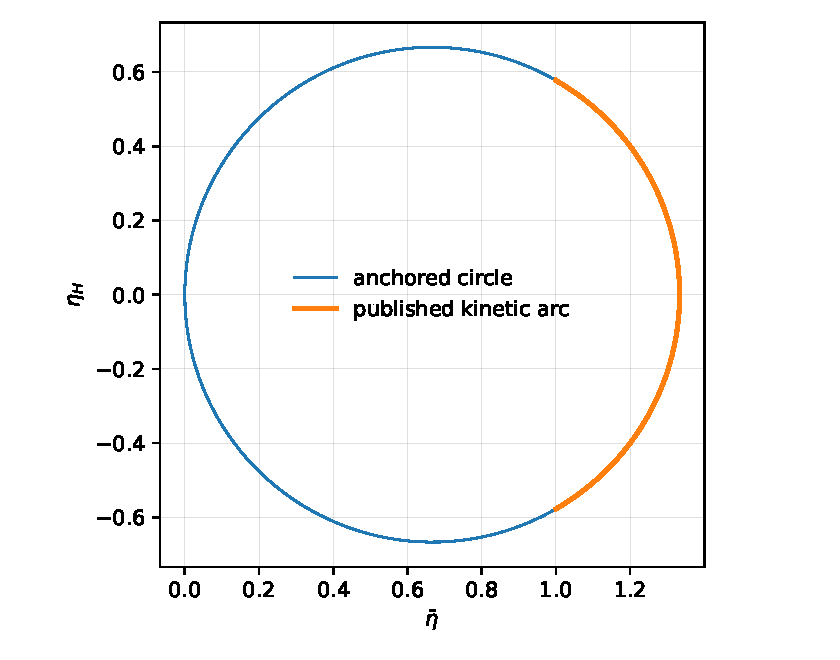
\includegraphics[width=.72\textwidth]{fhp_transport_circle.pdf}
\caption{Analytic molecular chaos response arc at $\rho=3$, generated directly from \cref{eq:kin_coeffs}. The thin curve is the complete anchored circle from \cref{eq:kin_circle_centered}; the thicker curve is the interval traced by $p\in[0,1]$. This is an analytic figure, not simulation data.}
\label{fig:fhp_circle}
\end{figure}

\section{Complex spectral form}
The same geometry is more informative when written as a complex response
\begin{equation}
 Z_B=\bar\eta+i\eta_H.
 \label{eq:zb_def}
\end{equation}
The shear sector eigenvalue of the published molecular chaos collision matrix can be written in the conventions used by the test suite as
\begin{equation}
 \lambda=-\frac{D}{2}+i\frac{\sqrt3 D}{3}d.
 \label{eq:kin_lambda}
\end{equation}
Direct inversion gives
\begin{equation}
 Z_B=-\frac{1}{4\lambda^*}.
 \label{eq:kin_spectral}
\end{equation}
The real part of $\lambda$ is $-D/2$ and is independent of $p$ at fixed density. As $p$ varies, $\lambda$ therefore moves on a vertical line in the complex plane. Conjugation and multiplication by a nonzero scalar preserve the line structure, and complex inversion maps a line not through the origin to a circle through the origin. The transport circle is thus the inverse image of dissipative spectral flatness in this kinetic model.

This observation is stronger conceptually than the completed square. It identifies which part of the eigenvalue produces the circle. The imaginary part carries the chirality dependent reactive coordinate. The fixed real part sets the circle. If correlations renormalize only the imaginary part of the effective inverse response, the circle survives. If they introduce chirality dependence into the real part, the anchored circle is broken.

\section{Exact finite verification in $\mathbb{Q}(\sqrt3)$}
The test \texttt{tests/test\_transport\_circle.py} avoids floating point arithmetic. Every quantity is represented as $r+s\sqrt3$ with rational $r$ and $s$. The test evaluates eleven density values, sixty five chirality values, and five weak field values, for a total of
\begin{equation}
 \HXTransportGridPoints{}
 \label{eq:transport_grid_count}
\end{equation}
parameter triples. At every point it checks the zero field circle, \cref{eq:kin_spectral}, and the stated weak field transformed circle exactly.

The CRTC package contains a separate zero field grid. It evaluates densities $\rho=n/16$ for $n=1,\ldots,95$ and chirality values $p=m/100$ for $m=0,\ldots,100$. This gives
\begin{equation}
 95\times101=\CRTCBoltzmannGridPoints{}
 \label{eq:crtc_boltz_grid_count}
\end{equation}
exact rational points. The test checks the polynomial circle identity at every point. The two counts are not alternative reports of the same run. They cover different finite parameter sets and test overlapping but not identical statements.

These finite checks do not prove the continuum relation. The proof is the algebra in \cref{eq:kin_circle_shifted}. Their role is to verify that the executable formulas, sign conventions, lattice shift, field transformation, and spectral relation agree with the symbolic derivation across broad finite domains.

\section{Weak field transformation}
The HX89 transport test also implements the weak field image given in the cited model. In the test conventions, with $b=B/2$ and scale $1+b^2$, the pair $(\eta,\eta_H)$ is transformed by a scaled rotation. The lattice shift must be carried through the same complex factor. Once that shift is handled consistently, the image of the zero field circle is again a circle with the correspondingly transformed center and radius.

The point of this test is bookkeeping as much as physics. A coordinate shift that is applied to shear viscosity at zero field but forgotten after a complex rotation can create a spurious circle defect. Exact arithmetic makes such a mismatch visible immediately. The thesis therefore treats the shifted coordinate $\bar\eta$ as part of the response definition whenever the Boltzmann formula is used.

\section{Relation to the inverse response classifier}
The kinetic circle can be put directly into the closure free language developed in \cref{ch:rigidity}. From \cref{eq:kin_spectral},
\begin{equation}
 \frac{1}{Z_B}=-4\lambda^*.
 \label{eq:kin_inverse_z}
\end{equation}
Hence
\begin{equation}
 \RePart\!\left(\frac{1}{Z_B}\right)=2D,
 \label{eq:kin_inverse_real}
\end{equation}
which is independent of $p$ at fixed density. The published kinetic circle is therefore a direct instance of inverse response rigidity.

This formulation also shows why a fixed prefactor should not be treated as fundamental. If one writes $Z=A_1/(\alpha+i\beta)$ with a parameter dependent residue $A_1(p)$, it is the ratio $\alpha/A_1$ that appears in the measured inverse response. The classifier should be applied to $1/Z$ itself. It does not require an assumption that a kinetic overlap or susceptibility prefactor remains unrenormalized.

\section{What this chapter proves}
The chapter proves three statements conditional only on the cited kinetic formulas:
\begin{enumerate}[label=\alph*)]
\item eliminating the chirality parameter produces the circle \cref{eq:kin_circle_eta};
\item the complex response is the inverse of the conjugate shear eigenvalue up to the stated factor, \cref{eq:kin_spectral};
\item the finite executable representations agree with those identities over their declared exact domains.
\end{enumerate}

It does not prove that the fully correlated automaton has the same transport coefficients. Molecular chaos enters before \cref{eq:kin_coeffs}; algebra performed afterward cannot remove that premise. The distinction becomes central in \cref{ch:discussion}.

\section{Chapter conclusion}
The published chiral FHP kinetic transport circle is an exact geometric image of a vertically flat shear eigenvalue locus. This gives a concrete model in which dissipative flatness and reactive chirality produce a circle by complex inversion. The result suggests the correct structural variable for a correlated theory: not the raw shear and Hall viscosities separately, but the real part of their measured inverse complex response. The next chapter proves that this observation is in fact an exact equivalence for any nonzero response, independent of the kinetic closure.
